\documentclass[12pt]{article}
\usepackage[spanish]{babel}
\usepackage[utf8]{inputenc}
\usepackage[framemethod=TikZ]{mdframed}
\usepackage[a4paper, margin = 1.5cm]{geometry}
\usepackage{amsmath}
\usepackage{amssymb}
\usepackage{amsthm}
\usepackage{graphics}
\usepackage{subfigure}
\usepackage{lipsum}
\usepackage{array}
\usepackage{multicol, multirow}
\usepackage{enumerate}
\usepackage{tikz}
\usepackage{pgffor}
\usepackage{ifthen}
\usepackage{enumitem}
\usepackage{hyperref}
\usepackage{listings}
\usepackage{titlesec}  
\usepackage{titletoc}  
\usepackage{longtable}
\usepackage{booktabs}
\usepackage{eso-pic} % <- Marca de agua


% Configuración del índice
\contentsmargin{0cm}
\dottedcontents{section}[1.5cm]{\contentslabel{2.0cm}}{1.5cm}{0pc}
\dottedcontents{subsection}[3.8cm]{\contentslabel{2.5cm}}{3.2cm}{0pc}

%Gestión de Hipervínculos
\hypersetup{
    colorlinks=true,
    linkcolor=blue,
    filecolor=magenta,      
    urlcolor=cyan,
    bookmarksopen=true
}

% --- Gestión marca de agua --- 
\AddToHook{shipout/foreground}{
    \begin{tikzpicture}[remember picture,overlay]
        \node at (current page.center){
            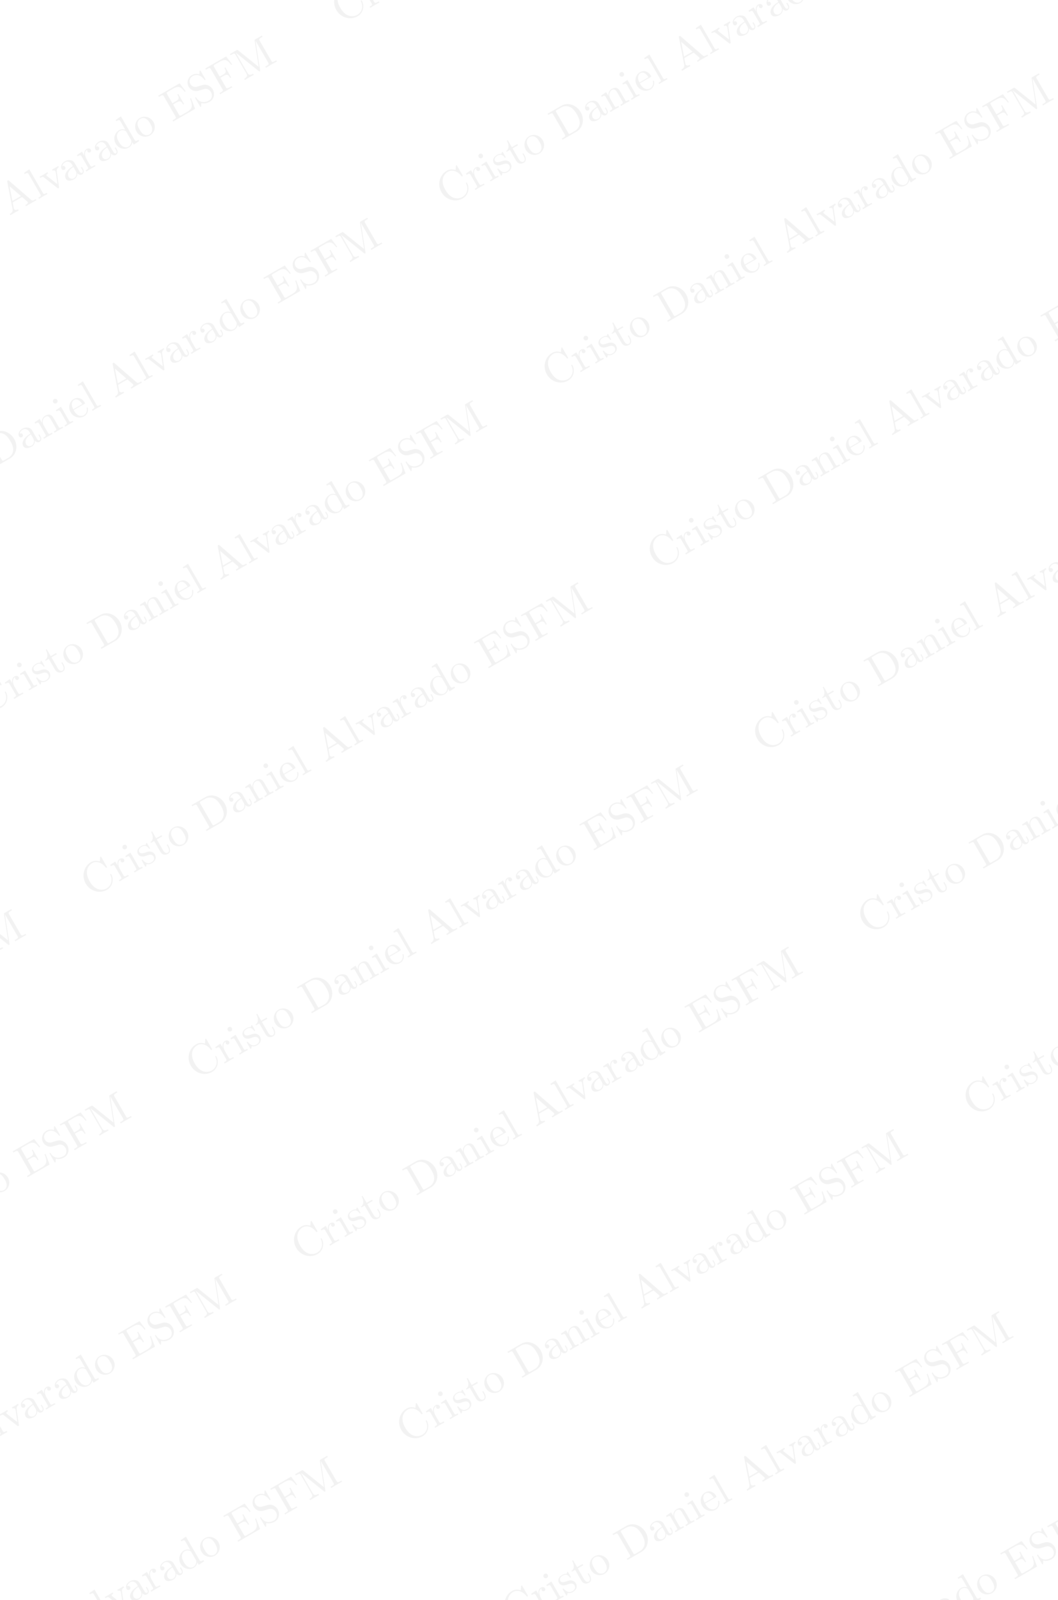
\includegraphics[width=\paperwidth,height=\paperheight,keepaspectratio]{watermark-1.png}
        };
    \end{tikzpicture}%
}


%Gestión de Código de Programación
\definecolor{listing-background}{HTML}{F7F7F7}
\definecolor{listing-rule}{HTML}{B3B2B3}
\definecolor{listing-numbers}{HTML}{B3B2B3}
\definecolor{listing-text-color}{HTML}{000000}
\definecolor{listing-keyword}{HTML}{435489}
\definecolor{listing-keyword-2}{HTML}{1284CA}
\definecolor{listing-keyword-3}{HTML}{9137CB}
\definecolor{listing-identifier}{HTML}{435489}
\definecolor{listing-string}{HTML}{00999A}
\definecolor{listing-comment}{HTML}{8E8E8E}

\lstdefinestyle{myStyle}{
    language         = Java,
    numbers          = none,
    xleftmargin      = 2.7em,
    framexleftmargin = 2.5em,
    backgroundcolor  = \color{gray!10},
    basicstyle       = \color{listing-text-color}\linespread{1.0}\ttfamily,
    breaklines       = true,
    frameshape       = {RYR}{Y}{Y}{RYR},
    rulecolor        = \color{black},
    tabsize          = 2,
    numberstyle      = \color{listing-numbers}\linespread{1.0}\small\ttfamily,
    aboveskip        = 1.0em,
    belowskip        = 0.1em,
    abovecaptionskip = 0em,
    belowcaptionskip = 1.0em,
    keywordstyle     = {\color{listing-keyword}\bfseries},
    keywordstyle     = {[2]\color{listing-keyword-2}\bfseries},
    keywordstyle     = {[3]\color{listing-keyword-3}\bfseries\itshape},
    sensitive        = true,
    identifierstyle  = \color{listing-identifier},
    commentstyle     = \color{listing-comment},
    stringstyle      = \color{listing-string},
    showstringspaces = false,
    label            = lst:bar,
    captionpos       = b,
}

\lstset{style = myStyle}

% Configuración correcta de secciones
\titleformat{\section}
  {\normalfont\Large\scshape}{\S\thesection}{1em}{}[\titlerule]
\titleformat{\subsection}
  {\normalfont\large\scshape}{\S\thesubsection}{1em}{}[\titlerule]

%Redefiniciones de comandos
\def\proof{\paragraph{Demostración:\\}}
\def\endproof{\hfill$\blacksquare$}

\def\sol{\paragraph{Solución:\\}}
\def\endsol{\hfill$\square$}

%Definiciones para enlistar
\newtheoremstyle{largebreak}
  {}% use the default space above
  {}% use the default space below
  {\normalfont}% body font
  {}% indent (0pt)
  {\bfseries}% header font
  {}% punctuation
  {\newline}% break after header
  {}% header spec

\theoremstyle{largebreak}

\newmdtheoremenv[
    leftmargin=0em,
    rightmargin=0em,
    innertopmargin=0pt,
    innerbottommargin=5pt,
    hidealllines = true,
    roundcorner = 5pt,
    backgroundcolor = gray!60!red!30
]{exa}{Ejemplo}[section]

\newmdtheoremenv[
    leftmargin=0em,
    rightmargin=0em,
    innertopmargin=0pt,
    innerbottommargin=5pt,
    hidealllines = true,
    roundcorner = 5pt,
    backgroundcolor = gray!50!blue!30
]{obs}{Observación}[section]

\newmdtheoremenv[
    leftmargin=0em,
    rightmargin=0em,
    innertopmargin=0pt,
    innerbottommargin=5pt,
    rightline = false,
    leftline = false
]{theor}{Teorema}[section]

\newmdtheoremenv[
    leftmargin=0em,
    rightmargin=0em,
    innertopmargin=0pt,
    innerbottommargin=5pt,
    rightline = false,
    leftline = false
]{propo}{Proposición}[section]

\newmdtheoremenv[
    leftmargin=0em,
    rightmargin=0em,
    innertopmargin=0pt,
    innerbottommargin=5pt,
    rightline = false,
    leftline = false
]{cor}{Corolario}[section]

\newmdtheoremenv[
    leftmargin=0em,
    rightmargin=0em,
    innertopmargin=0pt,
    innerbottommargin=5pt,
    rightline = false,
    leftline = false
]{lema}{Lema}[section]

\newmdtheoremenv[
    leftmargin=0em,
    rightmargin=0em,
    innertopmargin=0pt,
    innerbottommargin=5pt,
    roundcorner=5pt,
    backgroundcolor = gray!30,
    hidealllines = true
]{mydef}{Definición}[section]

\newmdtheoremenv[
    leftmargin=0em,
    rightmargin=0em,
    innertopmargin=0pt,
    innerbottommargin=5pt,
    roundcorner=5pt
]{excer}{Ejercicio}[section]

%Comandos personalizados
\newcommand\abs[1]{\ensuremath{\left|#1\right|}}
\newcommand\divides{\ensuremath{\bigm|}}
\newcommand\cf[3]{\ensuremath{#1:#2\rightarrow#3}}
\newcommand\contradiction{\ensuremath{\#_c}}
\newcommand\natint[1]{\ensuremath{\left[\big|#1\big|\right]}}
\newcounter{figcount}
\setcounter{figcount}{1}

% Configuración avanzada del índice
\usepackage{titletoc}
\usepackage{etoolbox}

% Estilo moderno para el índice
\contentsmargin{0cm}
\dottedcontents{part}[-1cm]{}{0cm}{}

% Estilo para secciones
\titlecontents{section}
  [0em]
  {\vspace{0.2ex}\large}
  {\makebox[2em][l]{\large\S\thecontentslabel}\hspace*{0.5em}}
  {}
  {\titlerule*[0.6em]{\textperiodcentered}\bfseries\contentspage}
  [\vspace{0.4ex}]

% Estilo para subsecciones
\titlecontents{subsection}
  [2.5em]
  {\vspace{0.2ex}\normalsize}
  {\makebox[3em][l]{\large\S\thecontentslabel}\hspace*{0.5em}}
  {}
  {\titlerule*[0.5em]{\textperiodcentered}\contentspage}
  [\vspace{0.3ex}]

%Texto Listado de Código

\renewcommand{\lstlistingname}{Código}
\renewcommand{\lstlistlistingname}{Lista de \lstlistingname s}

\begin{document}
    \setlength{\parskip}{5pt}
    \setlength{\parindent}{12pt}
    \title{Programación Orientada a Objetos}
    \author{Cristo Alvarado}
    \maketitle

    \begin{abstract}
        Ejemplo Abstract.
    \end{abstract}
    
    \tableofcontents

    \lstlistoflistings

    \section{Fundamentos}

    \subsection{¿Qué es la POO?}

    \begin{mydef}[\textbf{Paradigma de Programación}]
        Un \textbf{paradigma de programación} es \textit{una manera o estilo de programación de software}. Se trata de un \textit{conjunto de métodos sistemáticos aplicables en todos los niveles del diseño de programas para resolver problemas computacionales}.
    \end{mydef}

    Básicamente, es una forma de pensar sobre cómo estructurar y escribir el código. Cada paradigma de programación ofrece diferentes tipos de enfoces/filosofías/reglas para abordar tareas específicas.

    Existen varios paradigmas de programación, algunos de los más comunes son los siguientes:

    \begin{exa}[\textbf{Paradigma Imperativo}]
        Este paradigma se \textit{basa en la ejecución secuencial de instrucciones, donde el programador especifica cada paso que la computadora debe realizar para lograr un resultado}. Incluye lo siguiente: 
        \begin{itemize}
            \item \textbf{Programación estructurada}.
            \item \textbf{Programacion Procedural}.
            \item \textbf{Programación Modular}.
        \end{itemize}
        Lenguajes como C, C++, y Java pueden ser utilizados bajo este paradigma.
    \end{exa}

    \begin{exa}[\textbf{Paradigma Orientado a Objetos}]
        En el \textbf{Paradigma Orientado a Objetos} (también llamado \textbf{Programación Orientada a Objetos} y abreviado \textbf{POO}) se \textit{construyen modelos de objetos que representan elementos (objetos) del problema a resolver, que tienen características y funciones}. Permite \textit{separar los diferentes componentes de un programa, simplificando así su creación, depuración y posteriores mejoras}. La programación orientada a objetos \textit{disminuye los errores y promociona la reutilización del código. Es una manera especial de programar, que se acerca de alguna manera a cómo expresaríamos las cosas en la vida real}.

        Lenguajes de programación orientados a objetos son Java, Python o C\#.
    \end{exa}

    \begin{obs}[\textbf{Objetos}]
        En el paradigma orientado a objetos, \textit{podemos definir un objeto como una estructura abstracta que, de manera más fiable, describe un posible objeto del mundo real y su relación con el resto del mundo que lo rodea a través de interfaces}.
    \end{obs}

    La programación orientada a objetos se sirve de diferentes conceptos como:
    \begin{itemize}
        \item \textbf{Abstracción de datos}
        \item \textbf{Encapsulación}
        \item \textbf{Eventos}
        \item \textbf{Modularidad}
        \item \textbf{Herencia}
        \item \textbf{Polimorfismo}
    \end{itemize}

    La programación orientada a objetos tiene varias ventajas:
    \begin{itemize}
        \item POO es más fácil y rápida de ejecutar.
        \item POO provee una estructura clara de los programas.
        \item POO ayuda a mantener la filosofía del código Java DRY \textit{``Don't Repeat Yourself''}, y hace que el código sea más fácil de mantener, modificar y debuggear.
        \item POO hace posibel crear aplicaciones totalmente reusables con menos código y menos tiempo de desarrollo.
    \end{itemize}

    \begin{obs}[\textbf{Filosofía DRY}]
        La filosofía DRY trata sobre la repetición del código. En vez de repetir un código, se debe intentar reutilizar el mismo cada que sea posible.
    \end{obs}

    \subsection{Clases y Objetos}

    Dos aspectos fundamentales de la POO son las \textbf{clases} y los \textbf{objetos}.

    \begin{mydef}[\textbf{Clase}]
        En POO, una \textbf{clase} es una \textit{plantilla o modelo que define las propiedades y comportamientos comunes de un conjunto de objetos}. Es \textit{en esencia una plantilla de lo que será un objeto}.
    \end{mydef}

    Una clase \textit{puede contener atributos (variables) y métodos (funciones) que describen el estado y el comportamiento de los objetos que se crean a partir de ella}.

    \begin{mydef}[\textbf{Objeto}]
        En POO, un \textbf{objeto} es una \textit{instancia de una clase}.
    \end{mydef}

    Cada objeto \textit{tiene su propio estado y comportamiento, que se define por la clase a la que pertenece}. Los objetos \textit{son entidades concretas que se crean a partir de las clases y pueden interactuar entre sí}.

    \begin{mydef}[\textbf{Instancia}]
        Una \textbf{instancia} es \textit{un objeto específico creado a partir de una clase}.
    \end{mydef}

    \begin{exa}[\textbf{Clases y Objetos}]
        La siguiente tabla muestra ejemplos de clases y objetos:
        \begin{longtable}{c c}
            \toprule
            \toprule
            \textbf{Clase} & \textbf{Objeto} \\
            \midrule
            \midrule
            \endfirsthead
            
            \midrule
            \midrule
            \textbf{Clase} & \textbf{Objeto} \\
            \midrule
            \midrule
            \endhead
            
             \multirow{3}{*}{Fruta} & Manzana \\  
            & Plátano \\
            & Mango \\
            \hline

            \multirow{3}{*}{Carro} & Volvo EX30 \\  
            & Audi A3 \\
            & Toyota C-HR \\

            \bottomrule
            \bottomrule
        \end{longtable}
        Básicamente las clases son plantillas que definen las características y comportamientos de los objetos, mientras que los objetos son instancias concretas de esas clases.
    \end{exa}

    Cuando los objetos individuales son creados a partir de una clase, ellos heredan todas las variables y métodos de la clase.

    \begin{obs}[\textbf{Java y POO}]
        Todo en Java está asociado con clases y objetos, junto con sus métodos y variables.
    \end{obs}
    
    En la vida real un carro tiene \textbf{atributos}, como el color y su tamaño, y \textbf{métodos}, como aceleara y frenar.

    \begin{obs}[\textbf{Declaración de Clases en Java}]
        Para declarar una clase en Java usamos la palabra reservada \lstinline|class|:
        \begin{lstlisting}[caption={Declaración de Clase en Java.},label=DescriptiveLabel]
    public class Ejemplo{
        int x = 5;
    }
        \end{lstlisting}
        Siempre el nombre de la clase debe comenzar con mayúsculas y debe ser el mismo que el nombre del archivo.
    \end{obs}

    Como se mencionaba anteriormente en Java un objeto es creado a partir de una clase.

    \begin{obs}[\textbf{Creación de Objetos en Java}]
        Para crear un objeto debemos especificar el nombre de la clase seguido del nombre del objeto, y luego usar la palabra reservada \lstinline|new|, como se muestra a continuación:
        \begin{lstlisting}[caption={Declaración de Objeto en Java.},label=DescriptiveLabel]
public class Main {
    int x = 5;
    public static void main(String[] args) {
        Main myObj = new Main();
        System.out.println(myObj.x);
    }
}
        \end{lstlisting}
    \end{obs}

    También es posible crear múltiples objetos de la misma clase:

    \begin{lstlisting}[caption={Declaración de Objeto en Java.},label=DescriptiveLabel]
public class Main {
    int x = 5;
    public static void main(String[] args) {
        Main myObj1 = new Main();
        Main myObj2 = new Main();
        System.out.println(myObj1.x);
        System.out.println(myObj2.x);
    }
}
    \end{lstlisting}

    También podemos usar múltiples clases en y acceder a alguna de ella a la otra clase. Esto es usado comumnente para la organización de clases (una clase tiene todos los atributos y métodos, mientras que la otra clase tiene el método \lstinline|main()|).

    \begin{exa}
        En este ejemplo tenemos dos clases, \lstinline|Main| y \lstinline|Second|:
        \begin{lstlisting}[caption={Archivo con la Clase \lstinline|Main|.},label=DescriptiveLabel]
class Main {
    int x = 10;
    public static void main (String[] args){
        Second segunda = new Second();
        System.out.println("El numero de la clase Second es: " + segunda.x);
    }   
}
        \end{lstlisting}
        y,
        \begin{lstlisting}[caption={Archivo con la Clase \lstinline|Second|.},label=DescriptiveLabel]
public class Second {
    int x = 20;
}
        \end{lstlisting}
        Al ejecutar el código anterior, la ejecución mostrará el número \lstinline|20|.
    \end{exa}

    \subsection{Atributos}

    En los ejemplos anteriores nombramos a \lstinline|x| como una variable, pero realmente esta es un \textbf{atributo} de la clase. 

    \begin{mydef}[\textbf{Atributo}]
        En POO, un \textbf{atributo} es una \textit{característica o propiedad de un objeto}.
    \end{mydef}

    


\end{document}